\section{Exercise 1a: Coherent Demodulation}
\label{sec:ex1a}

\subsection*{Objective}
Implement a coherent AM demodulator that recovers the baseband message in time and frequency domains.

\subsection*{Module Design}
The coherent demodulation sub-VI is shown in Figure~\ref{fig:coherent_vi}.
\begin{figure}[H]
\centering
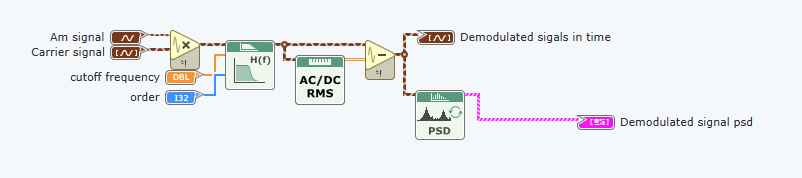
\includegraphics[width=\linewidth]{figures/Coherant_Demodulation_VI.png}
\caption{Block diagram of the coherent demodulation VI.}
\label{fig:coherent_vi}
\end{figure}

The implemented processing chain is:
\begin{enumerate}
\item Multiply the AM input signal by a local carrier at the same carrier frequency.
\item Apply a Butterworth low-pass filter (order and cutoff are exposed as controls).
\item Estimate the DC component and subtract it from the filtered waveform.
\item Display the recovered message in time domain and as a PSD estimate.
\end{enumerate}

\subsection*{Link to Theory}
From coherent detection theory (Section~\ref{sec:theory}), after multiplication and low-pass filtering,
\begin{equation}
y_{\mathrm{LPF}}(t)=\frac{1}{2}\left[A_c + A_m m(t)\right]\cos\phi,
\end{equation}
which includes:
\begin{itemize}
\item the desired baseband term proportional to $m(t)$,
\item a DC component proportional to $A_c$.
\end{itemize}
This directly explains why the VI needs both low-pass filtering and DC removal.

\subsection*{Why Low-Pass Filter, DC Removal, and Scaling Are Needed}
\begin{itemize}
\item \textbf{Low-pass filter:} removes components near $2f_c$ produced by the product detector.
\item \textbf{DC removal:} removes the carrier-dependent offset so the output is centered around zero.
\item \textbf{Amplitude scaling:} the demodulated message is attenuated (ideal factor $\approx 1/2$), so gain correction is required to match the original message amplitude.
\end{itemize}

\subsection*{Expected Output}
With correct carrier synchronization, the demodulated waveform is a sinusoid at $f_m$, and the demodulated PSD shows a dominant peak at the message frequency.
